\documentclass[11pt]{article}
\usepackage[utf8]{inputenc}
\usepackage[T1]{fontenc}
\usepackage{graphicx}
\usepackage[portuguese]{babel}
\usepackage{geometry}
\usepackage{listings}
\usepackage{hyperref}
\usepackage{bookmark}
\usepackage{float}
\graphicspath{ {./img/} }
\begin{document}

\title{Trabalho Prático 1 PDS}
\author{Nuno José Gomes Rodrigues a85207}
\maketitle

\tableofcontents

\pagebreak
\section{Introdução}

Este trabalho incide na alteração da frequência de amostragem por amostragem discreta de um sinal contínuo amostrado, transformada-z e filtros digitais. Para o efeito, será implementado um módulo em Matlab que permite fazer a sub amostragem de um sinal de áudio de forma a que a representação de este sinal amostrado ocupe menos memória e exija menos cálculos no seu processamento. Este é o método estudado de decimação.
Ao resultado desta decimação poderá ser necessário o uso de um filtro passa-baixo na eventualidade na ocorrência de "aliasing". No âmbito deste trabalho será utilizado o filtro elíptico e este terá as seguintes especificações:
\begin{itemize}
\item{Ripple na banda passante de 40 dB}
\item{Ripple na banda de rejeição de 60 dB}
\item{Largura de banda de transição de 20\% da banda passante.}
\end{itemize}
Quanto ao sinal utilizado, trata-se de um sinal áudio amostrado a 8kHz.
\pagebreak
\section{Conceitos teóricos}
\subsection{Amostragem}

Para um sinal poder ser processado digitalmente, este tem de ser amostrado a uma certa frequência, isto é, transformar um sinal contínuo em um sinal discreto. Este sinal discreto pode ser digitalmente armazenado e alterado.
\begin{figure}[!h]
\begin{center}
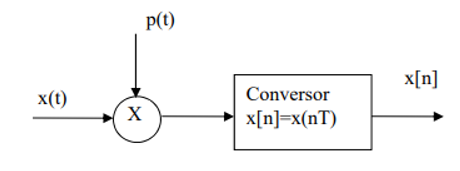
\includegraphics[width=7cm]{amostragem1.PNG}
\caption{Diagrama de blocos da Amostragem}
\label{figura1}
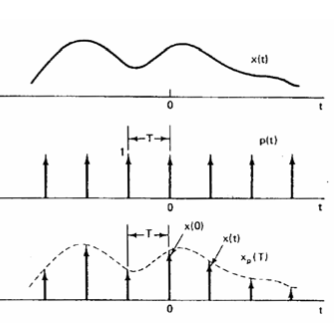
\includegraphics[width=7cm]{amostragem2.PNG}
\caption{Amostragem}
\label{figura2}
\end{center}
\end{figure}

A amostragem consiste na multiplicação do sinal por um trem de impulsos, tal como se pode ver na figura \ref{figura1}.
Na figura \ref{figura2} é possível ver o resultado desta multiplicação.
\subsection{Decimação}

Uma vez tendo obtido e armazenado a representação discreta do sinal parte-se para o processamento deste. Este processamento será muito pesado uma vez que está a ser realizado em toda a informação do sinal, o que geralmente não é necessário. Então, para baixar a memória que o sinal ocupa e a quantidade de processamento necessário, é feita a decimação do sinal, que consiste em reduzir o número de amostras deste por um fator N, ou seja, quanto maior o valor de N, menos amostras terá o sinal.
\begin{figure}[!h]
\begin{center}
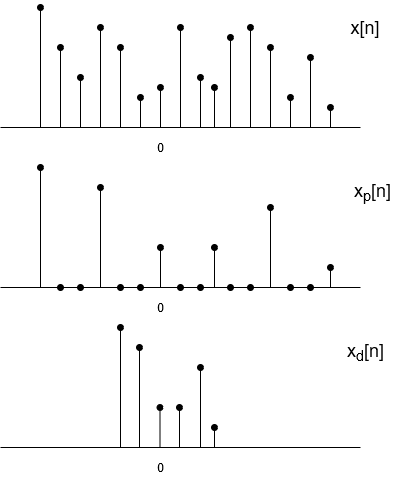
\includegraphics[width=7cm]{decimacao1.PNG}
\caption{Decimação no domínio dos tempos com fator N=3}
\label{figura3}
\end{center}
\end{figure}
\begin{figure}[!h]
\begin{center}
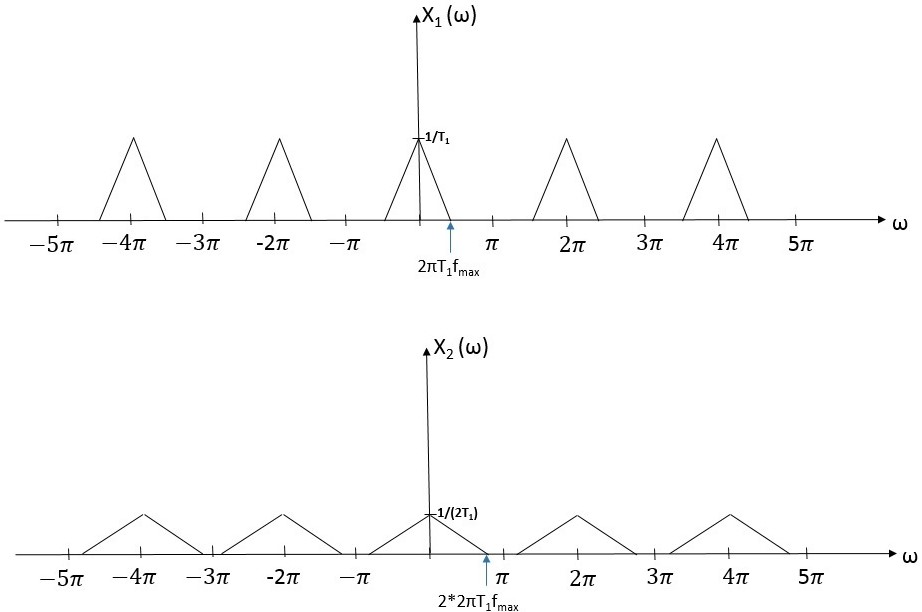
\includegraphics[width=8cm]{decimacao2.jpg}
\caption{Decimação no domínio das frequências sem ocorrencia de aliasing}
\label{figura4}
\end{center}
\end{figure}
\subsection{Aliasing}

Aquando à decimação pode ocorrer o fenómeno de "aliasing" que consiste na sobreposição do espetro de duas amostras diferentes. Estas sobreposições de espetros provocam distorções ao sinal que não permitirão que o sinal recuperado seja o sinal inicial.
\begin{figure}[h]
\begin{center}
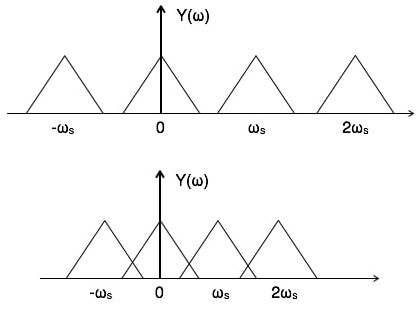
\includegraphics[width=8cm]{aliasing1.jpg}
\caption{Decimação no domínio das frequências com ocorrencia de aliasing}
\label{figura5}
\end{center}
\end{figure}

Segundo o teorema de Nyquist, para que não aconteça aliasing, a frequência de amostragem deve ser maior que duas vezes a maior frequência do sinal amostrado. Em termos ideais, para evitar o aliasing pode-se utilizar um filtro passa-baixo com frequência de corte de pi/N. Este filtro não é realizável devido à sua natureza não causal.
\newpage
\subsection{Filtro Elíptico}
\begin{figure}[h]
\begin{center}
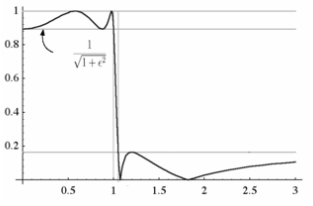
\includegraphics[width=8cm]{elitico1.png}
\caption{Diagrama de Amplitude de um Filtro Elíptico}
\label{figura5}
\end{center}
\end{figure}
\begin{itemize}
\item{A banda de transição do filtro elítico tem uma razão de N*20db/dec, sendo N a ordem do filtro e continua ainda depois de ws.}
\item{Ao contrário de outros filtros, o elíptico para além de possuir polos na banda de transição,possui também zeros.}
\item{Este filtro possui um polo imaginário colocado perto de Ws, o que faz aumentar o declive da banda de transição, precisando de menor ordem para obter resultados tão bons como outros filtros de ordens maiores.}
\item{Ao contrário de outros filtros, o filtro elíptico possui ripple na banda passante e na banda de rejeição. Se o ripple na banda passante for muito baixo, este filtro aproxima-se de um filtro Chebysheb tipo 2. Se o ripple na banda de rejeição foi muito baixo, este filtro aproxima-se de um filtro Chebysheb tipo 1. Se ambos os ripples forem muito baixos, aproxima-se de um filtro Butterworth.}
\item{A fase do filtro Elíptico é  muito pouco linear.}

\end{itemize}

\newpage
\section{Código Matlab}
\begin{figure}[h]
\begin{center}
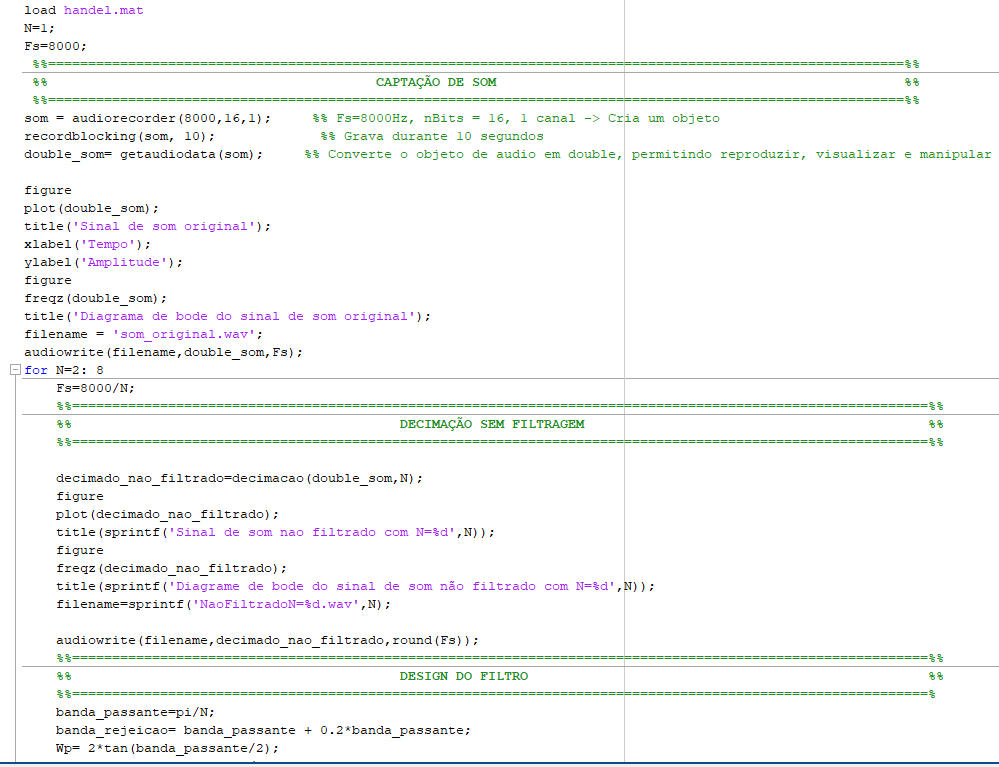
\includegraphics[width=17cm]{matlab1.png}
\end{center}
\end{figure}
\newpage
\begin{figure}[h]
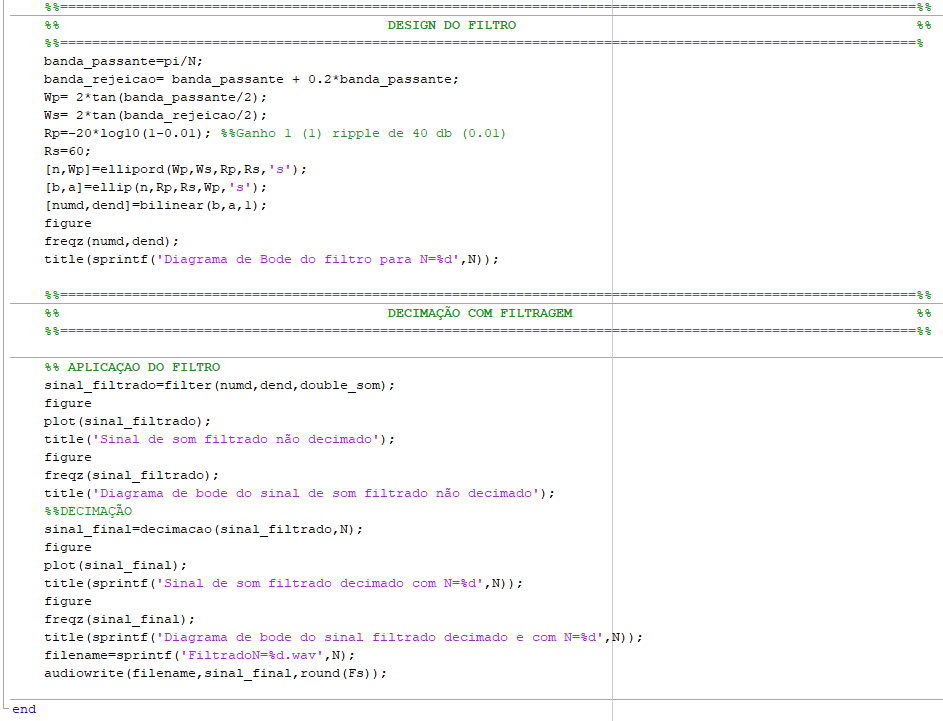
\includegraphics[width=16cm]{matlab2.png}
\\
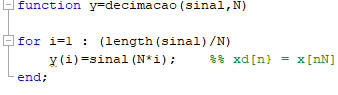
\includegraphics[width=7cm]{matlab3.png}
\end{figure}
\newpage
\section{Testes}
A amostra de som utilizada foi obtida diretamente pelo Matlab, recorrendo ao uso das seguintes funções: audiorecord, recordblocking e getaudiodata. Estas funções permitem respetivamente gravar som à frequência desejada, neste caso 8KHz, recolher amostra de som do tempo desejado, neste caso 10 segundos e passar o objeto de som para  uma variável manipulável pelo Matlab. Para melhor facilidade de reconhecimento de mudanças a nível audível, o som escolhido foi uma música, "Sleeping Dogs" de Zakk Wylde.
Inicialmente testou-se o som sem sub amostrar, de seguida testou-se o filtro, depois a sub amostragem do sinal de som, e finalmente a aplicação do filtro seguida da sub amostragem.
Para esse efeito, a frequência de Amostragem que inicialmente era de 8KHz, vai ser alterada a cada fator N de sub amostragem. Passa então a ser 8000/N.
\begin{figure}[h]
\begin{center}
\begin{minipage}[b]{0.45\linewidth}
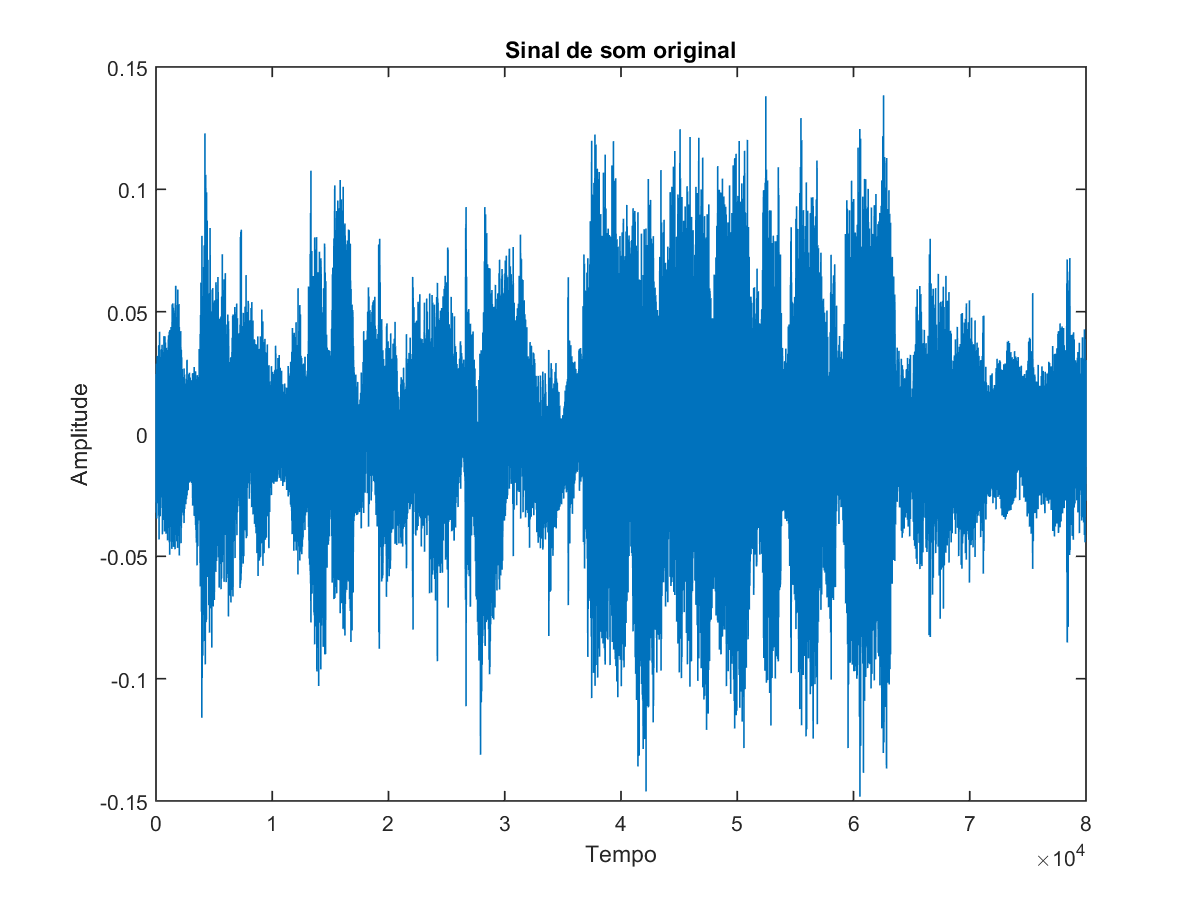
\includegraphics[width=7cm]{origis.png}
\caption{Sinal Original}
\label{figura6}
\end{minipage}
\begin{minipage}[b]{0.45\linewidth}
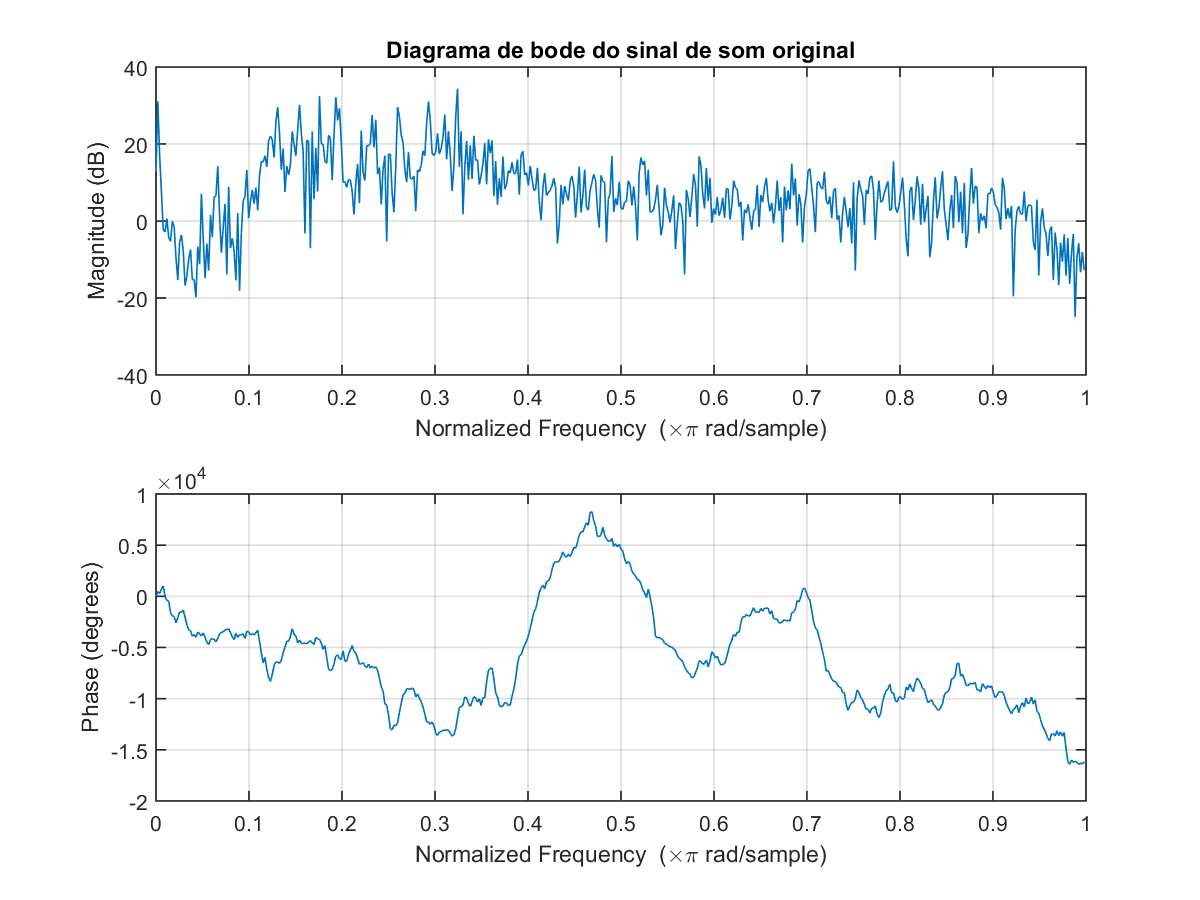
\includegraphics[width=7cm]{origib.png}
\caption{Diagrama de bode do Sinal Original}
\label{figura7}
\end{minipage}
\end{center}
\end{figure}
\newpage
\subsection{N=2}
\begin{figure}[h]
\begin{center}
\begin{minipage}[b]{0.45\linewidth}
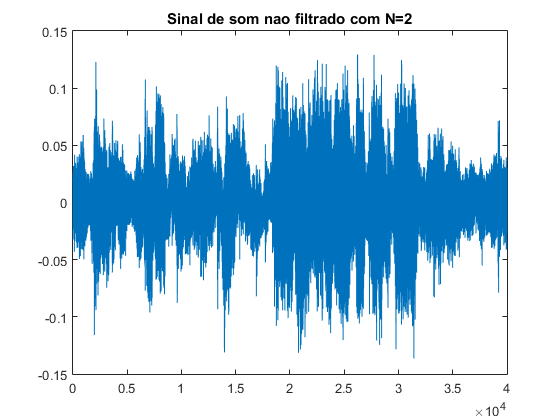
\includegraphics[width=7.5cm]{nfds2.png}
\caption{Sinal para N=2}
\label{figura8}
\end{minipage}
\begin{minipage}[b]{0.45\linewidth}
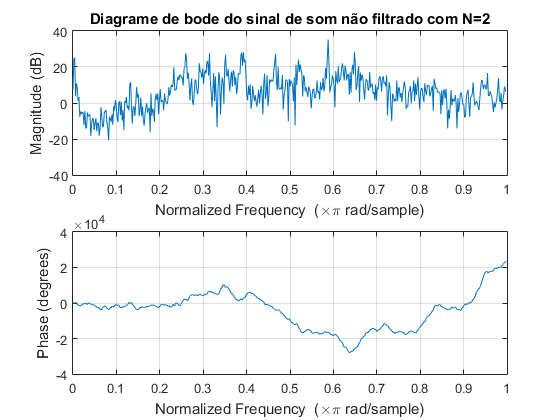
\includegraphics[width=7.5cm]{nfdb2.png}
\caption{Diagrama de bode para N=2}
\label{figura9}
\end{minipage}
\newline
\newline
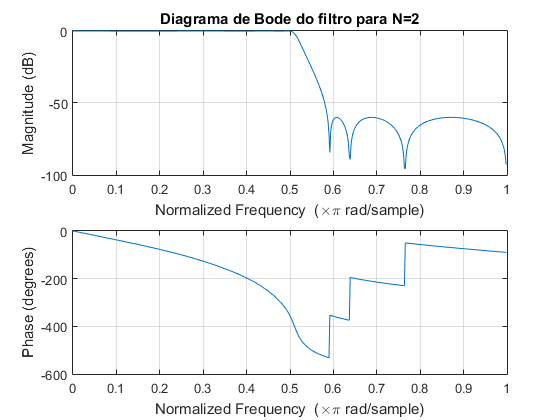
\includegraphics[width=8cm]{filtro2.png}
\caption{Diagrama de bode do filtro para N=2}
\label{figura10}
\end{center}
\end{figure}
\newpage
\begin{figure}[h]
\begin{center}
\begin{minipage}[b]{0.45\linewidth}
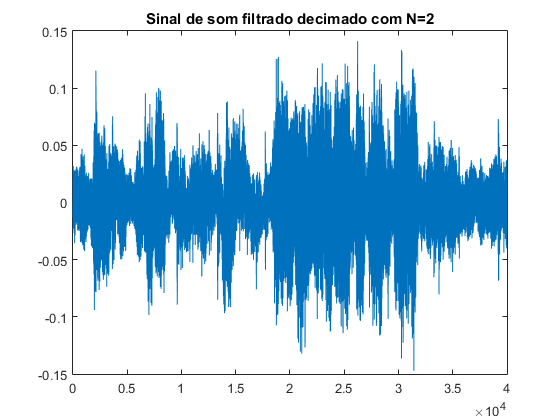
\includegraphics[width=7cm]{fds2.png}
\caption{Sinal Filtrado e sub amostrado com N=2}
\label{figura11}
\end{minipage}
\begin{minipage}[b]{0.45\linewidth}
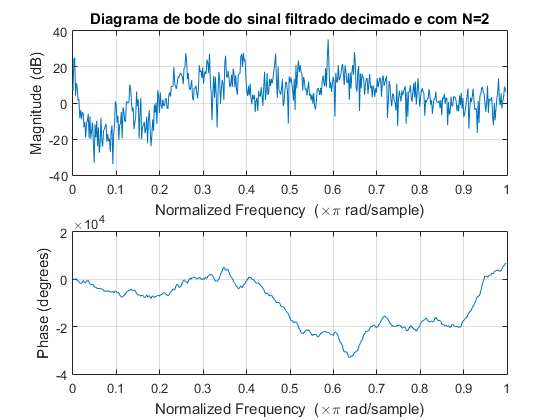
\includegraphics[width=7cm]{fdb2.png}
\caption{Diagrama de bode do Sinal filtrado e sub amostrado com N=2}
\label{figura12}
\end{minipage}
\end{center}
\end{figure}
Para o fator de decimação N=2, o sinal continua audível e agradável ao ouvido quer no sinal filtrado como no sinal não filtrado. As diferenças entre os dois sinais são pouco notórias. Todos os instrumentos se ouvem claramente. A diferença em relação ao sinal original é que para N=2 ambos os sinais têm um tom um pouco mais grave, quase como se estivessem a ser ouvidos como vindo debaixo de água.
\newpage
\subsection{N=3}
\begin{figure}[h]
\begin{center}
\begin{minipage}[b]{0.45\linewidth}
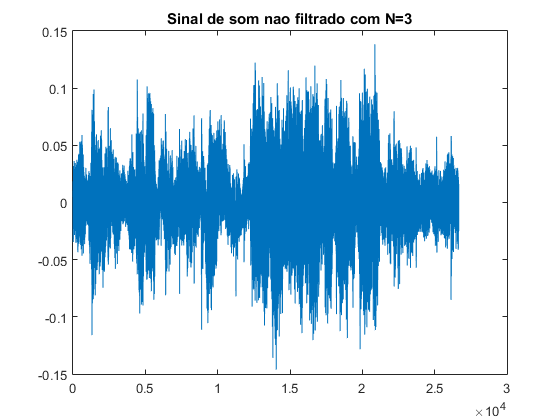
\includegraphics[width=7.5cm]{nfds3.png}
\caption{Sinal para N=3}
\label{figura8}
\end{minipage}
\begin{minipage}[b]{0.45\linewidth}
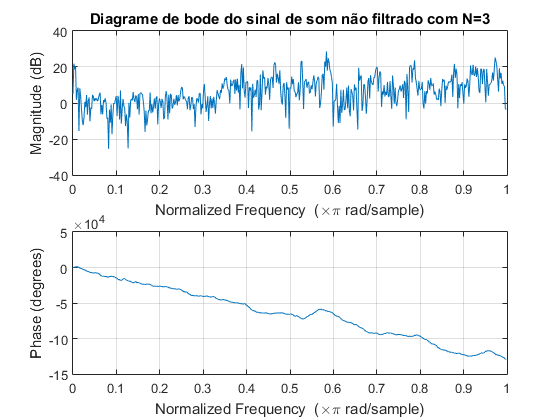
\includegraphics[width=7.5cm]{nfdb3.png}
\caption{Diagrama de bode para N=3}
\label{figura9}
\end{minipage}
\newline
\newline
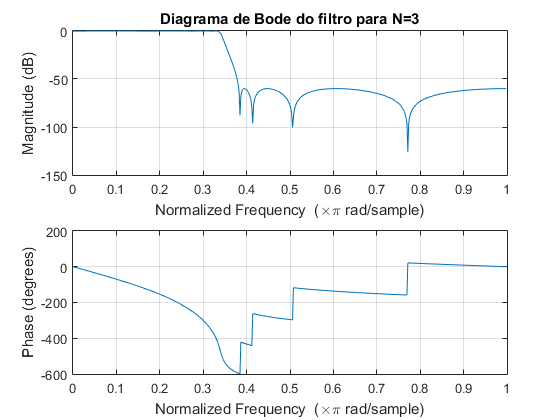
\includegraphics[width=8cm]{filtro3.png}
\caption{Diagrama de bode do filtro para N=3}
\label{figura10}
\end{center}
\end{figure}
\newpage
\begin{figure}[h]
\begin{center}
\begin{minipage}[b]{0.45\linewidth}
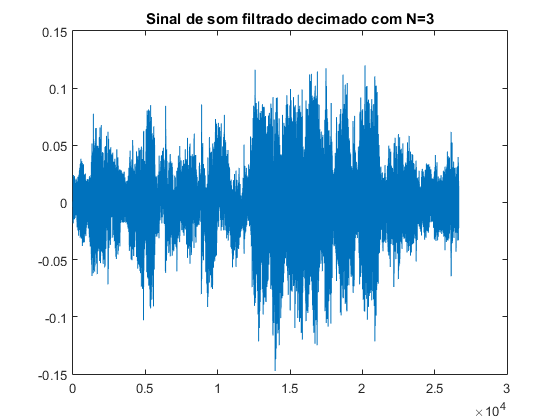
\includegraphics[width=7cm]{fds3.png}
\caption{Sinal Filtrado e sub amostrado com N=3}
\label{figura11}
\end{minipage}
\begin{minipage}[b]{0.45\linewidth}
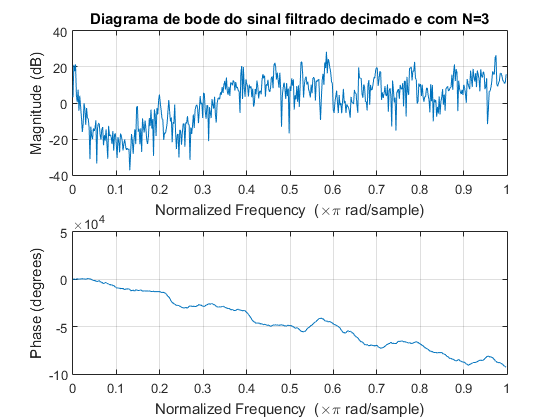
\includegraphics[width=7cm]{fdb3.png}
\caption{Diagrama de bode do Sinal filtrado e sub amostrado com N=3}
\label{figura}
\end{minipage}
\end{center}
\end{figure}
Para o fator de decimação N=3, começam a ser audíveis algumas diferenças entre o sinal filtrado e o sinal não filtrado. Ambos os sinais ficaram mais graves aparecendo algumas interferências no sinal não filtrado. A nível musical, no sinal não filtrado já não se conhece o som da guitarra, parecendo apenas um som de fundo e a letra passa a não ser percetível. Quanto ao sinal filtrado, todos os instrumentos se ouvem e a voz continua a ser reconhecível.
\newpage
\subsection{N=4}
\begin{figure}[h]
\begin{center}
\begin{minipage}[b]{0.45\linewidth}
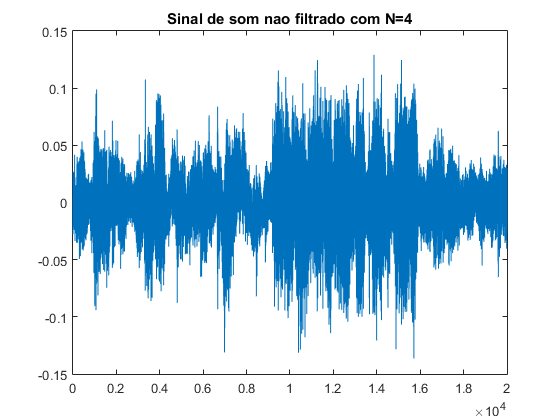
\includegraphics[width=7.5cm]{nfds4.png}
\caption{Sinal para N=4}
\label{figura8}
\end{minipage}
\begin{minipage}[b]{0.45\linewidth}
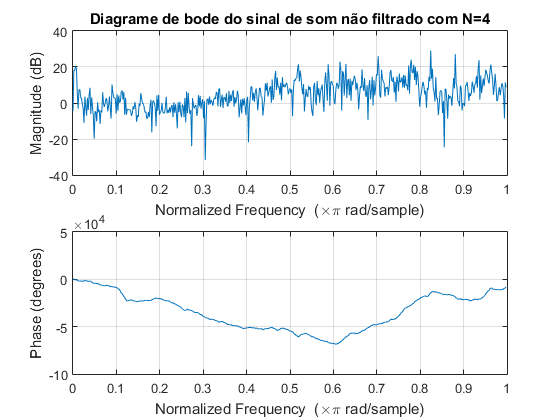
\includegraphics[width=7.5cm]{nfdb4.png}
\caption{Diagrama de bode para N=4}
\label{figura9}
\end{minipage}
\newline
\newline
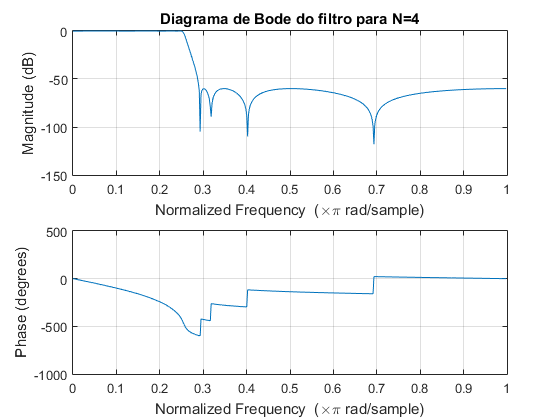
\includegraphics[width=8cm]{filtro4.png}
\caption{Diagrama de bode do filtro para N=4}
\label{figura10}
\end{center}
\end{figure}
\newpage
\begin{figure}[h]
\begin{center}
\begin{minipage}[b]{0.45\linewidth}
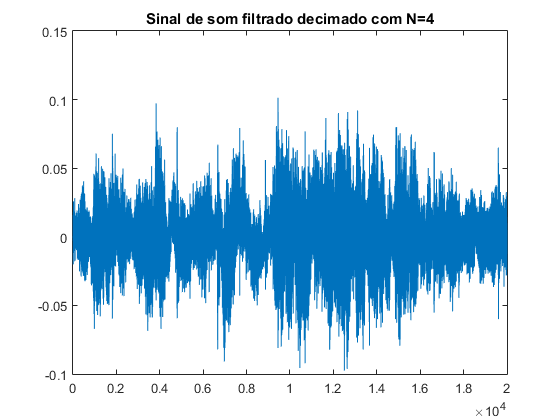
\includegraphics[width=7cm]{fds4.png}
\caption{Sinal Filtrado e sub amostrado com N=4}
\label{figura11}
\end{minipage}
\begin{minipage}[b]{0.45\linewidth}
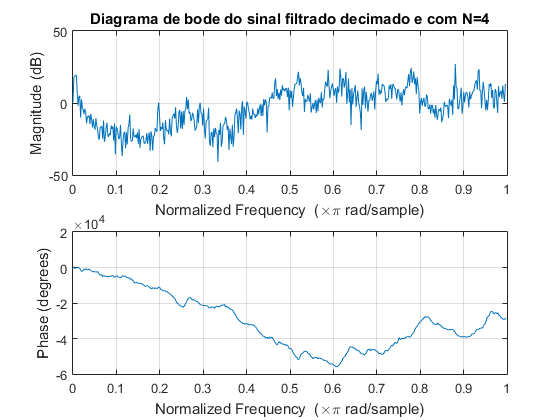
\includegraphics[width=7cm]{fdb4.png}
\caption{Diagrama de bode do Sinal filtrado e sub amostrado com N=4}
\label{figura}
\end{minipage}
\end{center}
\end{figure}
Para o fator de decimação N=4, as diferenças entre o sinal filtrado e não filtrado aumentam. O sinal não filtrado começa agora a ser não agradável ao ouvido visto que apresenta já bastante ruído. O sinal filtrado passa agora a ter uma parte aguda presente no seu todo, deixando também de ser agradável ao ouvido. A nível da música, no sinal não filtrado contínua a ouvir-se um pouco a voz ainda que não percetível e perdem-se algumas batidas da bateria no momento de maior intensidade musical. No  sinal filtrado continua a ser percetível a letra e a bateria, mas não a guitarra.

\newpage
\subsection{N=5}
\begin{figure}[h]
\begin{center}
\begin{minipage}[b]{0.45\linewidth}
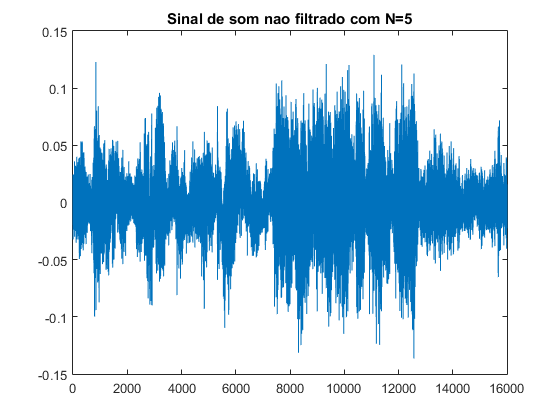
\includegraphics[width=7.5cm]{nfds5.png}
\caption{Sinal para N=5}
\label{figura8}
\end{minipage}
\begin{minipage}[b]{0.45\linewidth}
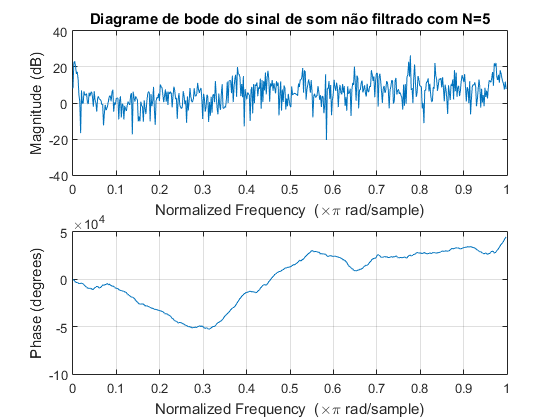
\includegraphics[width=7.5cm]{nfdb5.png}
\caption{Diagrama de bode para N=5}
\label{figura9}
\end{minipage}
\newline
\newline
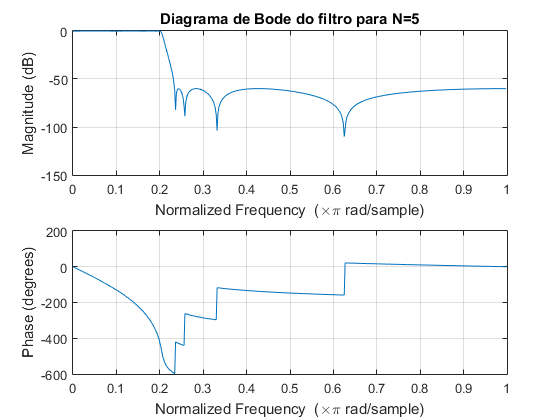
\includegraphics[width=8cm]{filtro5.png}
\caption{Diagrama de bode do filtro para N=5}
\label{figura10}
\end{center}
\end{figure}
\newpage
\begin{figure}[h]
\begin{center}
\begin{minipage}[b]{0.45\linewidth}
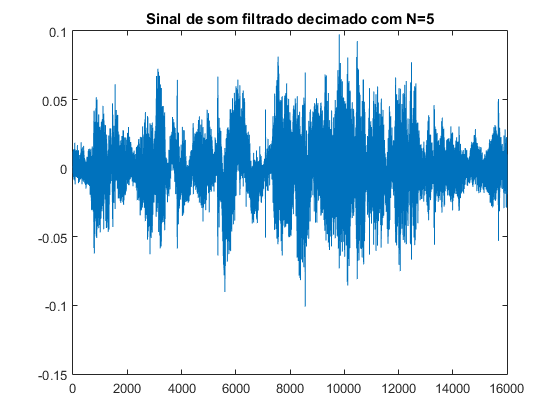
\includegraphics[width=7cm]{fds5.png}
\caption{Sinal Filtrado e sub amostrado com N=5}
\label{figura11}
\end{minipage}
\begin{minipage}[b]{0.45\linewidth}
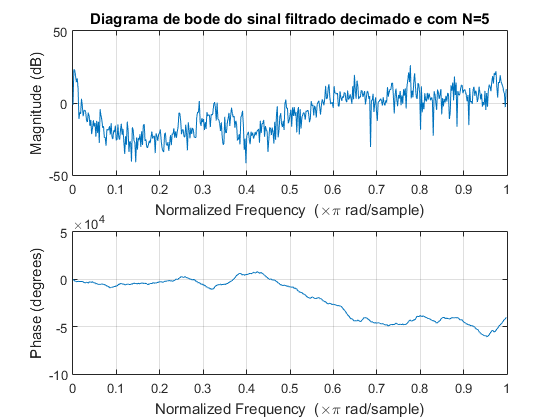
\includegraphics[width=7cm]{fdb5.png}
\caption{Diagrama de bode do Sinal filtrado e sub amostrado com N=5}
\label{figura}
\end{minipage}
\end{center}
\end{figure}
Para o fator de decimação N=5, as diferenças entre o sinal filtrado e não filtrado aumentam ainda mais. O sinal não filtrado ganha bastante ruído enquanto que o sinal filtrado perde agora a componente aguda que anteriormente tinha aparecido, ficando novamente agradável ao ouvido ainda que parecendo um pouco distante e como que estivesse debaixo de água. A nível musical, no sinal não filtrado apenas resta um pouco da melodia e poucas batidas da bateria, enquanto que no sinal filtrado a letra e a bateria continuam percetíveis e mantém grande parte da melodia.

\newpage
\subsection{N=6}
\begin{figure}[h]
\begin{center}
\begin{minipage}[b]{0.45\linewidth}
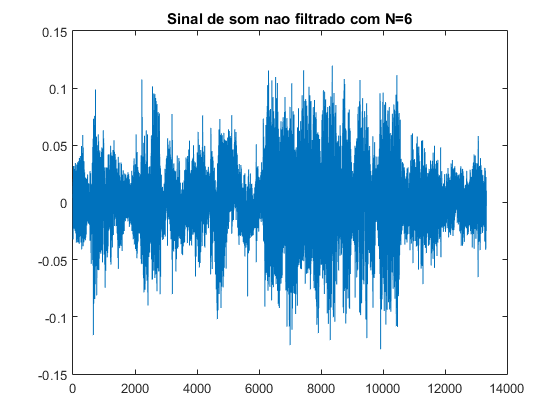
\includegraphics[width=7.5cm]{nfds6.png}
\caption{Sinal para N=6}
\label{figura8}
\end{minipage}
\begin{minipage}[b]{0.45\linewidth}
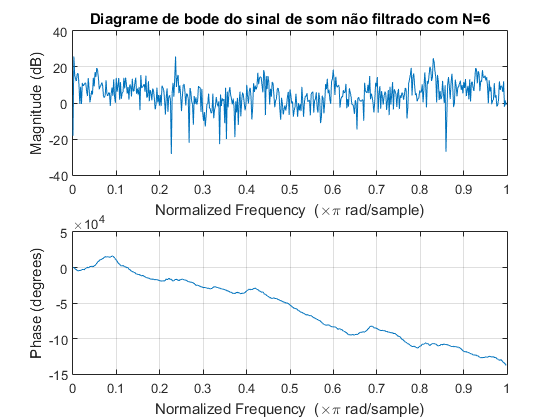
\includegraphics[width=7.5cm]{nfdb6.png}
\caption{Diagrama de bode para N=6}
\label{figura9}
\end{minipage}
\newline
\newline
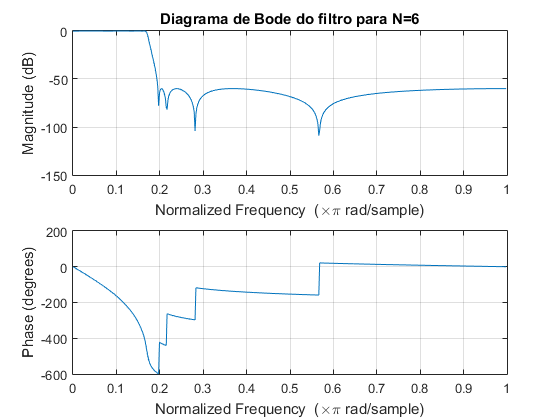
\includegraphics[width=8cm]{filtro6.png}
\caption{Diagrama de bode do filtro para N=6}
\label{figura10}
\end{center}
\end{figure}
\newpage
\begin{figure}[h]
\begin{center}
\begin{minipage}[b]{0.45\linewidth}
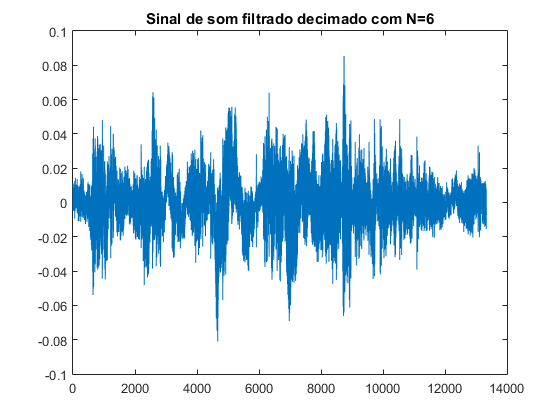
\includegraphics[width=7cm]{fds6.png}
\caption{Sinal Filtrado e sub amostrado com N=6}
\label{figura11}
\end{minipage}
\begin{minipage}[b]{0.45\linewidth}
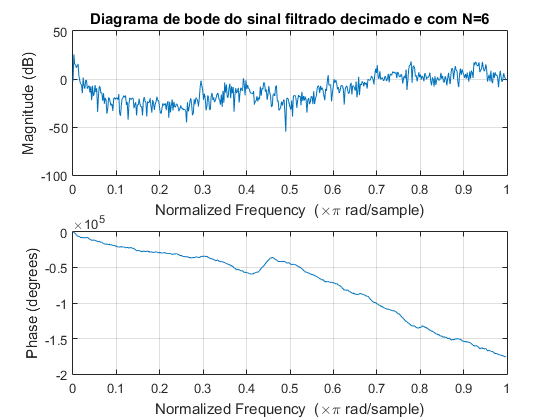
\includegraphics[width=7cm]{fdb6.png}
\caption{Diagrama de bode do Sinal filtrado e sub amostrado com N=6}
\label{figura}
\end{minipage}
\end{center}
\end{figure}
Para o fator de decimação N=6, o sinal não filtrado passa a ser maioritariamente ruído. O filtrado parece que está a ser ouvido a uma maior distância, voltando a aparecer uma pequena componente aguda na sua extensão. A nível musical,  o sinal não filtrado deixa de ser reconhecido como uma música devido à grande quantidade de ruído e já nem se conseguem ouvir as batidas da bateria. No sinal filtrado, ainda se ouve a bateria e a voz, mas a letras deixa de ser reconhecível.

\newpage
\subsection{N=7}
\begin{figure}[h]
\begin{center}
\begin{minipage}[b]{0.45\linewidth}
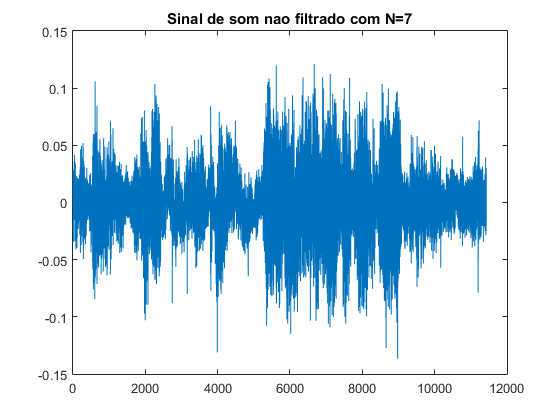
\includegraphics[width=7.5cm]{nfds7.png}
\caption{Sinal para N=7}
\label{figura8}
\end{minipage}
\begin{minipage}[b]{0.45\linewidth}
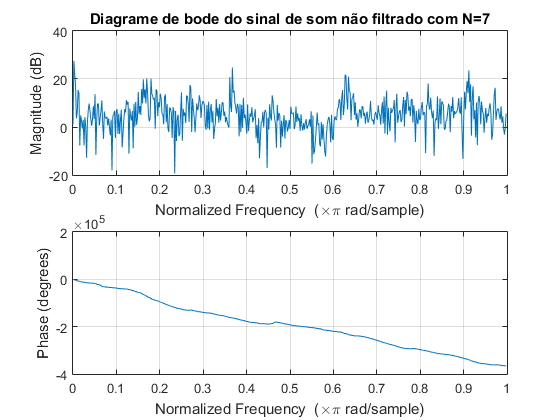
\includegraphics[width=7.5cm]{nfdb7.png}
\caption{Diagrama de bode para N=7}
\label{figura9}
\end{minipage}
\newline
\newline
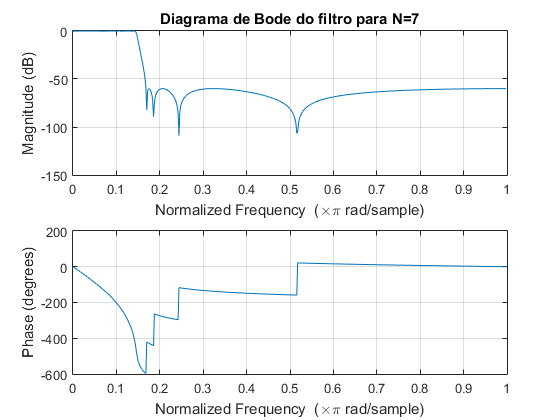
\includegraphics[width=8cm]{filtro7.png}
\caption{Diagrama de bode do filtro para N=7}
\label{figura10}
\end{center}
\end{figure}
\newpage
\begin{figure}[h]
\begin{center}
\begin{minipage}[b]{0.45\linewidth}
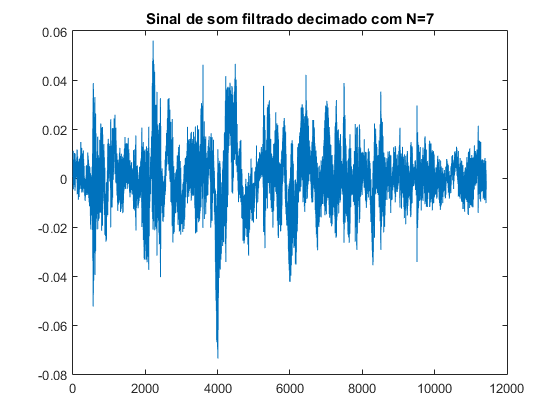
\includegraphics[width=7cm]{fds7.png}
\caption{Sinal Filtrado e sub amostrado com N=7}
\label{figura11}
\end{minipage}
\begin{minipage}[b]{0.45\linewidth}
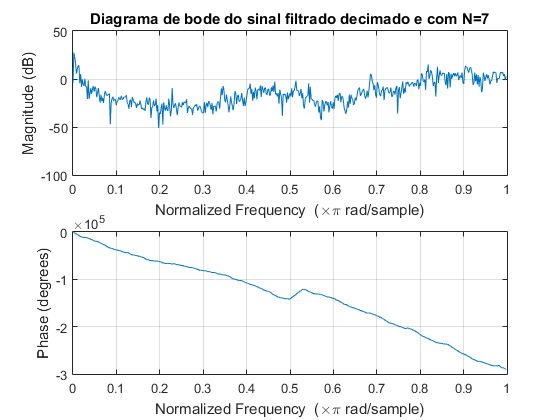
\includegraphics[width=7cm]{fdb7.png}
\caption{Diagrama de bode do Sinal filtrado e sub amostrado com N=7}
\label{figura}
\end{minipage}
\end{center}
\end{figure}
Para o fator de decimação N=7, o sinal não filtrado continua a ser composto por ruído enquanto o sinal filtrado perde bastante intensidade a nível auditivo comparativamente com o obtido em N=6. A nível musical, no sinal filtrado a melodia mantém-se embora que com um volume bastante mais baixo e parecendo mais distante. A voz e a bateria continuam a ser ouvidas.

\newpage
\subsection{N=8}
\begin{figure}[h]
\begin{center}
\begin{minipage}[b]{0.45\linewidth}
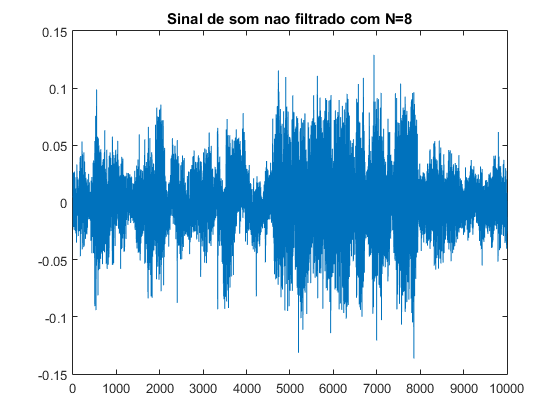
\includegraphics[width=7.5cm]{nfds8.png}
\caption{Sinal para N=8}
\label{figura8}
\end{minipage}
\begin{minipage}[b]{0.45\linewidth}
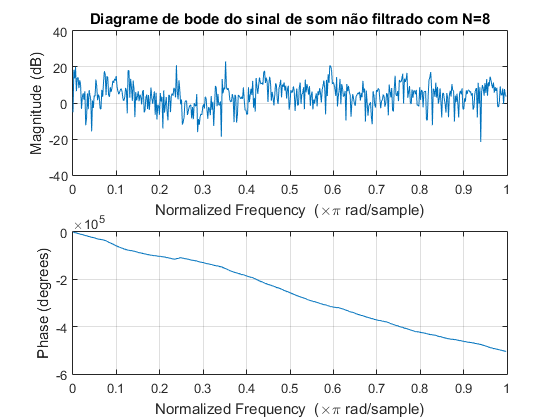
\includegraphics[width=7.5cm]{nfdb8.png}
\caption{Diagrama de bode para N=8}
\label{figura9}
\end{minipage}
\newline
\newline
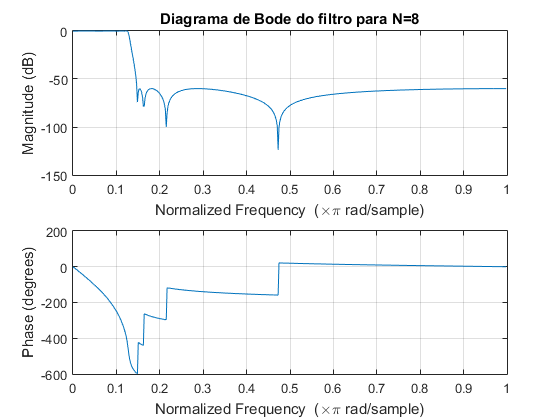
\includegraphics[width=8cm]{filtro8.png}
\caption{Diagrama de bode do filtro para N=8}
\label{figura10}
\end{center}
\end{figure}
\newpage
\begin{figure}[h]
\begin{center}
\begin{minipage}[b]{0.45\linewidth}
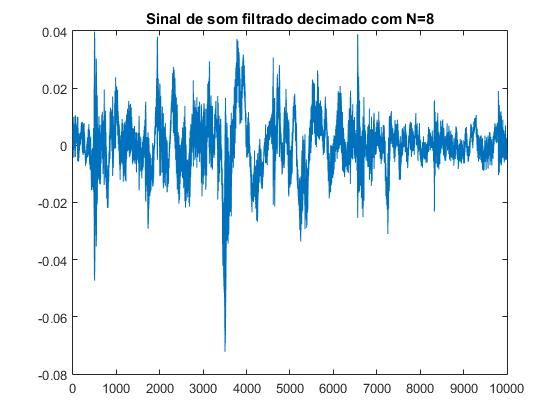
\includegraphics[width=7cm]{fds8.png}
\caption{Sinal Filtrado e sub amostrado com N=8}
\label{figura11}
\end{minipage}
\begin{minipage}[b]{0.45\linewidth}
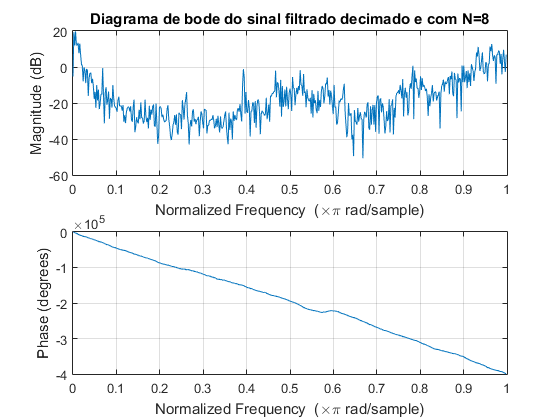
\includegraphics[width=7cm]{fdb8.png}
\caption{Diagrama de bode do Sinal filtrado e sub amostrado com N=8}
\label{figura}
\end{minipage}
\end{center}
\end{figure}
Para o fator de decimação N=8, o sinal não filtrado é quase constante, parecendo algum som debaixo de água a uma distância elevada, enquanto o sinal filtrado volta a perder novamente bastante intensidade. A nível musical, o sinal filtrado conta agora apenas com a melodia e algumas batidas da bateria, visto que a intensidade do som está demasiado baixa para que se consiga detetar a voz.
\newpage
\section{Conclusão}
Foi escolhida uma música como amostra de som já que apresenta uma maior variedade de frequências, permitindo assim um melhor estudo da decimação e do comportamento do filtro. \\
Foi possível concluir que à medida que com o incremento fator de decimação N, existia a ocorrencia de aliasing ficando cada vez mais informação do sinal sobreposta, gerando ruído.\\ Foi também possível concluir o filtro elíptico consegue prevenir a ocorrencia de aliasing quando aplicado ao sinal antes da decimação, mas à medida que o valor de N aumenta, a frequência de corte do filtro também tem de aumentar, o que resulta em perda de informação do sinal.\\
\newline
Com estes resultados, a conclusão final a que cheguei é que embora a decimação de um sinal o torne mais compacto a nível computacional e exija menos poder de processamento e cálculos, é necessário estabelecer um trade off entre estas facilidades e aquele que se deseja obter como resultado final, uma vez que para fatores de decimação elevados, a frequência de corte do filtro anti-aliasing será baixa, cortando muita informação do sinal.

\section{Repositório online}
De modo a melhor facilidade de acesso e para o professor poder aceder ao ficheiros de áudio resultantes deste trabalho, criei um repositório online público no github onde está presente todo o trabalho efetuado.
\newline
\href{https://github.com/sno0ker/TP1-PDS-85207}{https://github.com/sno0ker/TP1-PDS-85207}
\end{document}
